%!TeX program = xelatex
\documentclass[12pt,a4paper,UTF8]{ctexart}
\usepackage{zjureport}

%%-------------------------------正文开始---------------------------%%
\begin{document}

%%-----------------------封面--------------------%%
\cover
\clearpage

%%------------------摘要-------------%%
\pagenumbering{Roman}
\thispagestyle{empty}
\begin{abstract}
转座元件（transposable elements, TEs）占据人类基因组的重要部分，并通过插入、重排、调控元件供给和转录调控等方式参与基因组演化与疾病相关过程\cite{lander2001human,cordaux2009retrotransposons,chuong2017regulatory,bourque2018ten}。然而，TE 相关证据通常分散在基因组注释、表达数据、文献摘要、疾病关联和人工整理的知识条目中，研究者难以在同一界面内追踪“TE--分子实体--疾病--文献证据”的完整证据链。本 proposal 以已经实现的 TE-KG 本地 pilot resource 为基础，提出一个面向 TE 疾病机制研究的知识图谱资源建设方案。当前 \texttt{tekg3} 运行时已经由 Neo4j、PHP API、浏览器 G6 图谱、MySQL 表达摘要和 PubMed 元数据增强流程共同支撑；只读检查确认 live Neo4j 统计接口包含 11,415 个节点和 13,696 条关系，代表性 TE 条目 L1HS、AluJb 和 SVA 可解析。方案的核心假设是：若将 TE taxonomy、疾病关联、表达入口和 PubMed 证据元数据整合为可追踪、可导出、可验证的知识图谱，TE 相关机制假设的发现和证据审查将比孤立页面或人工检索更透明、更可复用。
\end{abstract}

%%--------------------------目录页------------------------%%
\clearpage
\tableofcontents

%%------------------------正文页从这里开始-------------------%
\clearpage
\pagenumbering{arabic}

\section{研究背景与科学问题}

TEs 不只是基因组中的重复序列负担。已有研究显示，逆转座元件和其他 TE 类群能够影响基因组结构、调控网络和物种演化\cite{cordaux2009retrotransposons,chuong2017regulatory,bourque2018ten}。在人类疾病研究中，TE 插入、TE 转录失控、TE 衍生调控元件和内源性逆转录病毒序列均可能与癌症、遗传病及其他病理过程相关\cite{burns2017cancer,payer2019genetic}。这些研究共同提出一个数据组织问题：TE 相关证据同时具有序列、分类、基因组位置、表达、疾病、功能和文献维度，单一表格或单一检索入口难以表达实体间关系。

知识图谱适合表示这种异质、关系密集的生物医学证据结构。已有生物医学知识整合工作表明，将多源实体和关系组织为可计算图谱，有助于复用既有知识并支持假设优先级排序\cite{himmelstein2017hetionet}。TE-KG 的科学问题因此可以表述为：如何把 TE 分类、疾病关联、表达证据和 PubMed 文献证据组织为一个可验证、可浏览、可导出的图谱资源，并避免把文献数量、期刊指标或自动化回答误写成未经验证的因果强度？

\section{核心假设与总体目标}

本 proposal 的核心假设是：一个以 Neo4j 为运行时核心、以 API contract 和浏览器 smoke test 为质量门禁、以 PubMed 元数据为证据层的 TE 知识图谱，可以为 TE 疾病机制研究提供比静态数据表更清晰的证据追踪能力。该假设不预设任一 TE--疾病关系为因果关系，而是把图谱关系、支持 PMID、期刊元数据覆盖率和前端证据表作为可审查的 evidence support。

总体目标是将当前 TE-KG pilot resource 发展为一个可公开、可复现、可审计的 TE 疾病知识图谱资源。具体目标包括：

\begin{enumerate}
    \item 建立以 \texttt{tekg3} 为唯一 runtime target 的图谱资源层，稳定表示 TE、疾病、功能、基因、蛋白、药物、文献等实体及其关系。
    \item 建立文献证据层，将 PubMed PMID、标题、期刊、年份、MeSH/关键词、作者、基金、化学物质和引用信息与既有 \texttt{Paper} 节点和 \texttt{BIO\_RELATION} 关系连接。
    \item 建立用户可审查的前端证据工作流，使研究者能够从图谱边跳转到 PubMed 证据表，并导出当前可见子图和所选边的证据 CSV。
    \item 建立开放数据与 FAIR 元数据计划，使代码、处理后数据、图谱导出、证据元数据和文档能够在许可允许范围内公开发布\cite{wilkinson2016fair,springer_nature_data_policy}。
\end{enumerate}

\section{已有基础与初步资源}

\subsection{运行时系统}

TE-KG 当前已经是一个本地 PHP + browser JavaScript + Neo4j + MySQL 系统。核心页面仍位于项目根目录，包括 \url{index.php}、\url{browse.php}、\url{preview.php}、\url{expression.php}、\url{expression_detail.php} 和 \url{path_finder.php}。主要运行时入口如下：

\begin{itemize}
    \item 图谱 API：\url{api/graph.php} 和 \url{api/graph_service.php}。
    \item Taxonomy API：\url{api/taxonomy.php}。
    \item Expression API：\url{api/expression_data.php}；\\
          \url{api/expression_repository.php}。
    \item Expression runtime 根目录：\url{data/bulk_expression_web}。
\end{itemize}

系统不再使用旧的 \url{data/raw/new_data/bulk_expression_web} 路径作为 expression runtime 根目录。

当前 live 检查确认，Neo4j 配置解析到 \texttt{tekg3}，\texttt{RETURN 1} 可执行，代表性 TE 名称 AluJb、L1HS 和 SVA 可解析。homepage stats API 以 Neo4j 为统计来源，报告当前运行时包含 11,415 个节点和 13,696 条关系。另一个 Neo4j 检查确认 225 个 \texttt{TE} 节点；该检查使用的 \texttt{BIO\_RELATION} 计数口径不同，因此正式规模表述以 live Neo4j 统计接口的节点和关系总数为主。

\subsection{文献证据与 2025 年影响因子元数据}

TE-KG 已经完成 PubMed 元数据增强流程。当前 PubMed PMID inventory 包含 2,308 个唯一 PMID，完整抓取写入 2,308 条 PubMed metadata records，失败数为 0。PubMed XML 提供 PMID、DOI、标题、摘要可用性、期刊、发表年份、发表类型、MeSH term、关键词、作者、单位、基金、化学物质和引用等字段；PubMed 本身不提供影响因子，影响因子必须来自外部期刊指标映射\cite{pubmed_ncbi}。

项目已将 2025 年影响因子元数据映射到现有 \texttt{Paper} 节点。映射结果显示，2,037 个 \texttt{Paper} 节点具有 2025 年影响因子元数据，271 个 \texttt{Paper} 节点保持 null / unmatched。该影响因子来源为项目内部批准的 \texttt{impact\_factor\_package\_2025}，不能表述为官方 JCR direct export。所有缺失值必须保留为 null、unknown 或 unmatched，不允许由模型或人工推断填补。

\subsection{图谱证据浏览与导出}

G6 图谱工作区已支持 evidence support UX。Graph API edge payload 包含 PMID 支持数、metric coverage、IF mean/max 等 \texttt{support\_*} 字段以及 eager evidence records。前端将边宽映射到 PMID 支持数，将边透明度映射到 metric coverage，并在边卡片中显示 PubMed evidence table。这里的 \texttt{support\_*} 字段只表示 evidence support，不表示 confidence。

图谱导出已支持当前可见子图的 nodes CSV、edges CSV 和 canvas PNG。SVG 导出尚未实现，界面仅保留 disabled 的 \texttt{SVG Soon} 状态。浏览器 smoke 当前通过 \texttt{LINE1} 查询；TE tree/load 回归检查确认 \texttt{LINE1} 动态图加载为 95 nodes / 103 edges，\texttt{L1HS} 动态图加载为 54 nodes / 58 edges，taxonomy tree 包含 1,632 nodes / 1,631 edges，并恢复了 L1HS 在 Class I / LINE 层级下的路径。

\begin{figure}[!htbp]
    \centering
    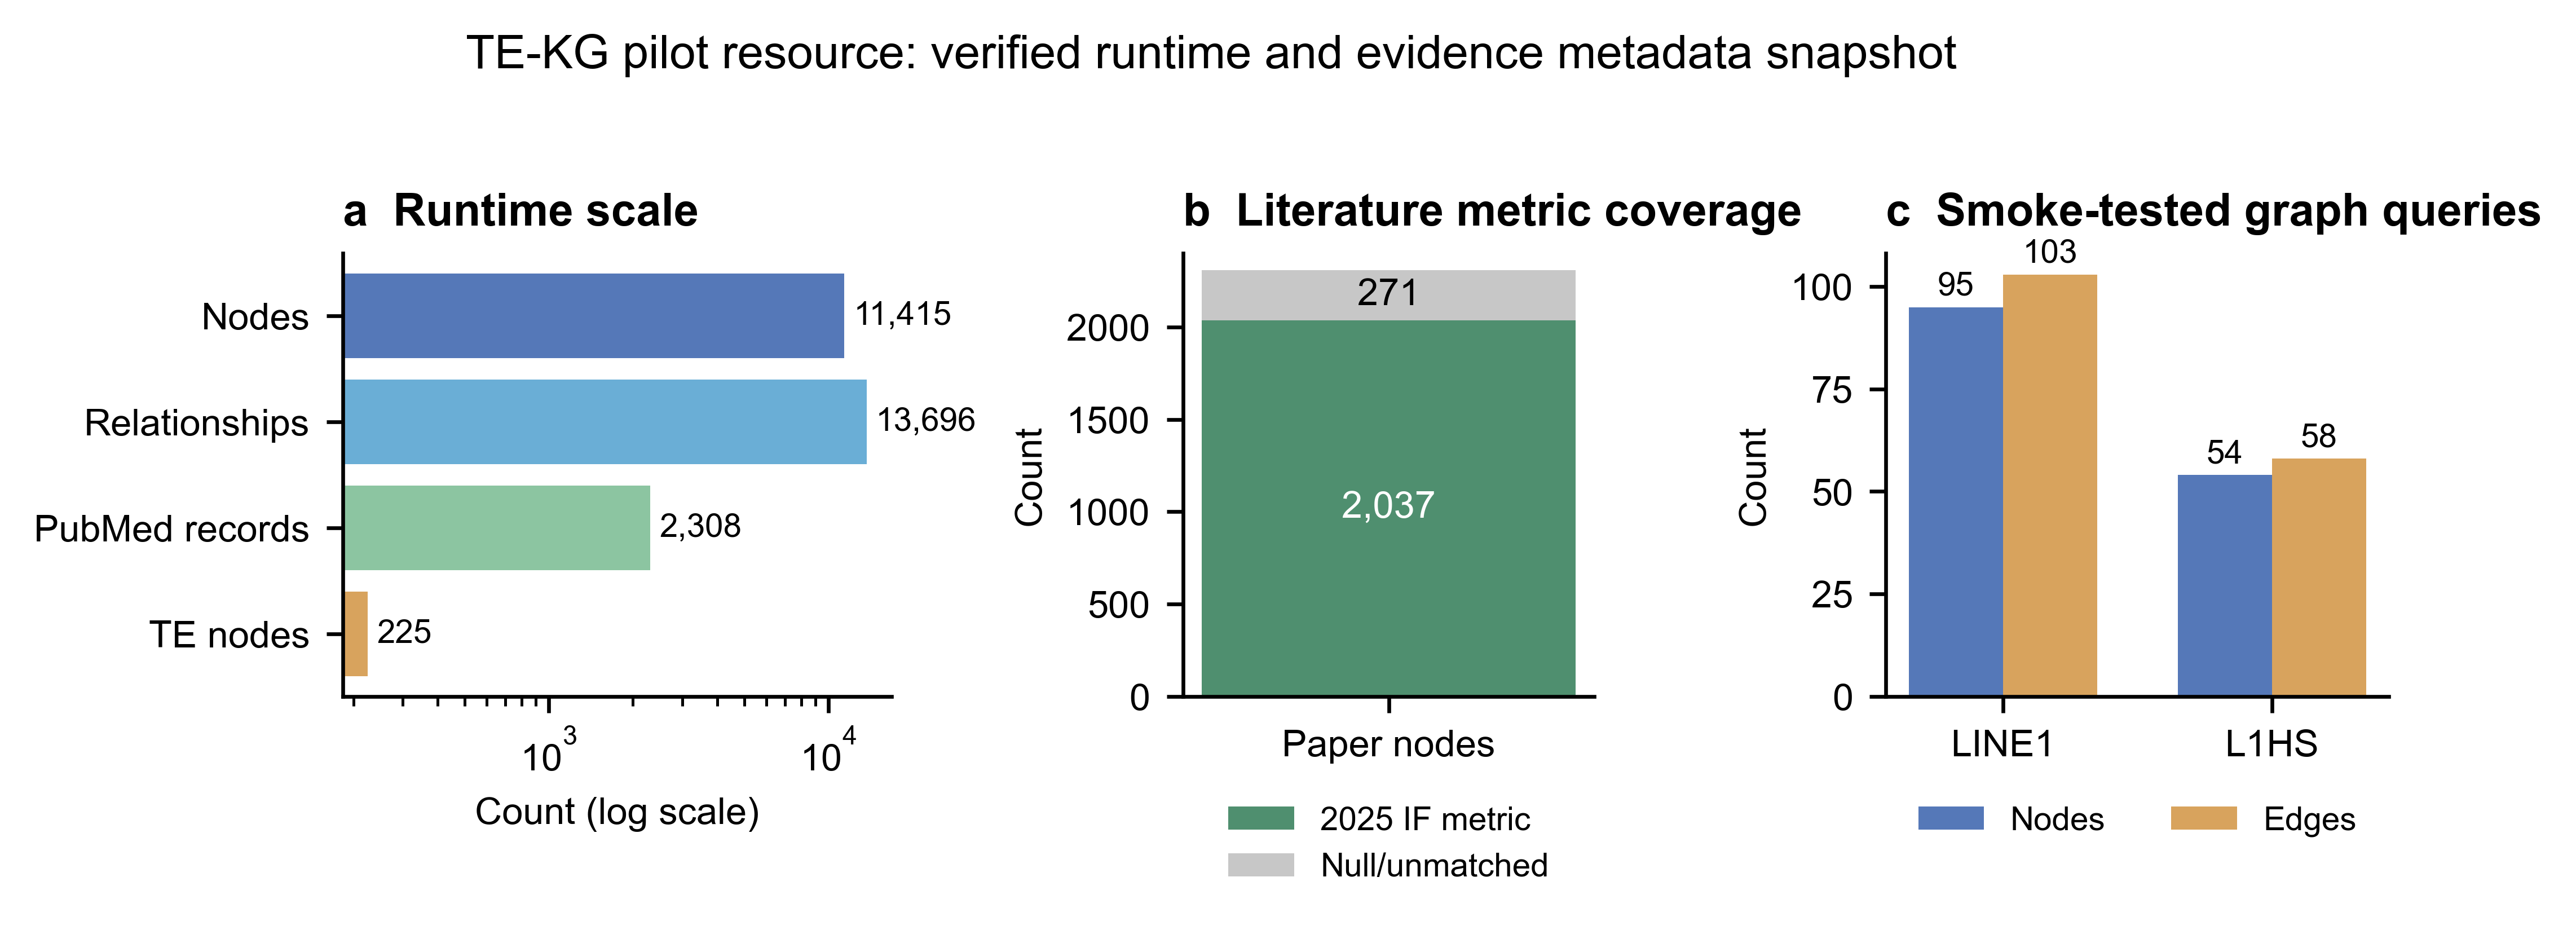
\includegraphics[width=\textwidth]{figures/tekg_resource_overview.png}
    \caption{TE-KG pilot resource 的当前运行时与证据元数据快照。Panel a 显示 live Neo4j 统计接口和 PubMed metadata pipeline 的主要规模；Panel b 显示 2025 年影响因子元数据在 \texttt{Paper} 节点上的 matched 与 null/unmatched 状态；Panel c 显示浏览器 smoke 覆盖的代表性图谱查询规模。图中数据来自本仓库当前只读检查和已归档完成计划，源表见 \texttt{docs/proposal/tekg\_proposal\_figure\_data.csv}。}
    \label{fig:tekg-overview}
\end{figure}

\section{研究内容与技术路线}

\subsection{Aim 1：巩固 TE-KG 运行时图谱与 API contract}

Aim 1 将把 \texttt{tekg3} 固化为 proposal 阶段的唯一 Neo4j runtime target，并继续以 \texttt{api/graph.php}、\texttt{api/graph\_service.php}、\texttt{api/taxonomy.php} 和 expression API 作为稳定入口。该目标的重点不是新增第二套 taxonomy truth source，而是维护当前 Neo4j/API canonical 规则。任何 taxonomy、expression 或 graph runtime 变更都应通过现有检查验证，包括 runtime DB config、API contracts、expression path consistency、G6 browser smoke 和 no legacy DB fallback。

\subsection{Aim 2：建立可审查的 TE--疾病文献证据层}

Aim 2 将以当前 PubMed metadata 和 2025 年影响因子映射为基础，继续完善 \texttt{Paper.pmid} 与 \texttt{BIO\_RELATION.pmids} 的证据连接。证据层应明确区分三类信息：第一，文献事实字段，如 PMID、标题、期刊、年份、MeSH term 和 DOI；第二，关系支持字段，如 PMID 支持数和 metric coverage；第三，外部期刊元数据，如 2025 年影响因子。只有第一类和第二类可以直接支撑“关系有文献记录”的表述，第三类只能作为期刊元数据展示，不能被写成关系可信度或因果强度。

\subsection{Aim 3：建立开放、可导出、可复用的用户工作流}

Aim 3 将围绕 \texttt{preview.php} 的图谱工作区形成可复用浏览工作流。用户应能够从 TE 或疾病节点出发，查看相关实体、展开局部邻域、检查边证据、下载可见子图 CSV/PNG，并保留所选边的 PubMed evidence table。Agent/DeepThink 子系统可作为实验性 evidence-grounded assistant workflow，用于研究型问题的证据包组织和报告草稿，但其输出必须经过 evidence package、evidence walk、report plan 和 integrity gate 约束。该 assistant layer 不应被描述为成熟自治科研代理。

\section{创新点}

本 proposal 的创新点在于把 TE 研究中常见的多个断裂层面连接为一个可审计的资源工作流。第一，图谱资源不只提供实体检索，而是把 TE taxonomy、疾病关联、表达入口和文献证据组织到同一运行时。第二，文献支持不是抽象分数，而是可展开的 PMID-level evidence records，研究者能够回到 PubMed 条目检查原始文献信息。第三，2025 年影响因子元数据被明确限制为期刊层面的辅助展示，避免将期刊指标误写成关系 confidence。第四，系统用可运行检查维护 runtime contract，使资源建设过程本身可审计。

\section{数据开放与 FAIR 计划}

TE-KG 的数据开放策略应遵循 FAIR 原则，即数据和元数据需要可发现、可访问、可互操作、可复用\cite{wilkinson2016fair}。在本 proposal 中，原则上可以公开的内容包括项目代码、API contract 文档、处理后的 PubMed metadata JSONL、图谱导出 CSV、可公开的 Neo4j 导出、图谱统计图源数据、检查脚本输出摘要和 proposal 文档本身。第三方或许可受限的数据源需要单独标注来源、许可和再分发限制。

Data Availability statement 的建议文本如下：

\tbox{
The TE-KG source code, processed graph-export tables, proposal figure source data and documentation are planned for public release in a versioned repository. Processed PubMed-derived metadata will be distributed with PMID-level provenance where redistribution is permitted. Third-party resources, including Repbase/RMSK-derived taxonomy inputs and the 2025 impact-factor package used for internal journal metadata mapping, will be released only when licensing permits; otherwise, accession routes, transformation scripts and null/unmatched records will be documented without redistributing restricted source files.
}

该声明仍需人工确认最终仓库地址、许可证、数据 DOI 或长期归档平台。若某些第三方输入不能公开，应公开 transformation scripts、字段说明、缺失值规则和可复现流程，而不是公开受限源文件。

\section{风险、边界与质量控制}

本 proposal 的主要风险来自三类边界。第一，taxonomy runtime truth source 仍需持续维护。当前 \texttt{api/taxonomy.php} contract 和 TE tree smoke 已通过，但 homepage taxonomy truth-source 检查提示 \texttt{index.php} 的 ring chart 仍需核查是否完全使用 Neo4j-backed helper。因此，在正式发布前应把 homepage taxonomy 展示与 runtime canonical source 对齐，或在论文/报告中排除该页面作为核心证据。

第二，文献证据和期刊指标必须避免过度解释。PubMed metadata 支持文献信息组织，不能自动证明关系因果性；2025 年影响因子只表示期刊层面元数据，不应参与 confidence 命名。关系边上的 \texttt{support\_*} 字段应保持 evidence support 语义。

第三，Agent/DeepThink 子系统仍处于实验性工作流阶段。已有 deterministic tests、live targeted plugin checks 和 evidence-walk integrity gate 支撑其可运行性，但 Phase 5C semantic proxy 不能验证生物医学事实，也不能证明 claim-level citation support。因此，proposal 中只把 Agent 写作层作为辅助证据组织与报告草稿工具，不把它作为成熟自治发现系统。

\section{预期成果}

本 proposal 的预期成果包括一个以 \texttt{tekg3} 为核心的 TE-KG pilot resource、一个 PubMed PMID-level 文献证据层、一个可导出可浏览的 G6 图谱工作区、一套 Data Availability / FAIR 元数据说明，以及一组可运行检查作为资源质量门禁。若这些目标完成，TE-KG 将能够支持研究者从 TE 实体进入疾病和功能关系，检查 PMID 支持，导出当前可见子图，并以透明方式区分“已有证据记录”“期刊元数据覆盖”和“仍需人工验证的机制解释”。

%%----------- 参考文献 -------------------%%
\reference

\end{document}
